%!TEX root = main.tex
\chapter{OBJEK DAN METODOLOGI PENELITIAN}

\section{Objek Penelitian}

Objek yang akan menjadi bahan kajian pada penelitian ini adalah sistem otentikasi atau sistem login pada mesin ATM. Sistem otentikasi pada mesin ATM yang ada sekarang menggunakan kartu dan PIN sebagai alat otentikasinya.

Proses otentikasi yang dilakukan sekarang adalah dengan memasukkan kartu ATM kedalam mesin kemudian mesin akan meminta otentikasi berupa PIN yang akan dimasukkan oleh pengguna melalui tombol yang ada pada mesin.

%Perangkat berupa mesin elektronik yang terhubung dengan pusat komputer layanan nasabah pada suatu lembaga penyimpan dana, sehingga dapat menggantikan sebagian fungsi kasir. Perangkat tersebut akan memungkinkan nasabah untuk melakukan transaksi dengan menggunakan suatu media baik berupa kartu atau media lainnya sebagai suatu identitas pengenal di dalam sistem. Jenis transaksi yang umum dilakukan melalui ATM antara lain berupa penarikan uang tunai dari rekening simpanan, pengecekan saldo, transfer kepada bank yang sama atau bank yang lain, serta pembayaran/pembelian berbagai barang/jasa.

\section{Metodologi Penelitian}

Metode pengembangan yang digunakan pada penelitian ini adalah metodologi standard pada pengembangan aplikasi yang menggunakan ekplorasi data yaitu \textit{CRoss InduStry Process for Data Mining} (CRISP-DM). CRIPS-DM digunakan karena kemampuan metologi tersebut yang dapat diterapkan kepada hampir semua jenis bisnis. Ada enam fase yang ada dalam metodologi ini yaitu \textit{Business Understanding}, \textit{Data Understanding},\textit{Data Preparation}, \textit{Modeling}, \textit{Evaluation} dan \textit{Deployment}.

\begin{figure}[h]
	\centering
	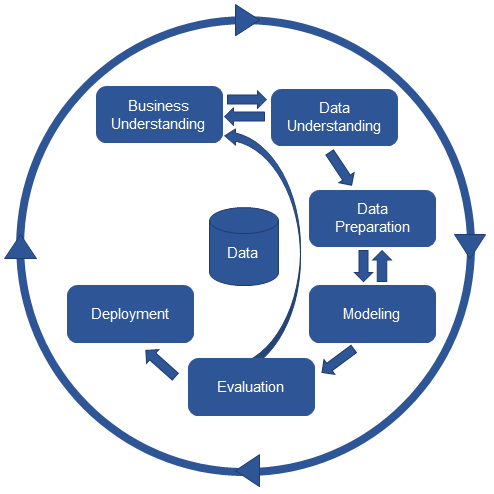
\includegraphics[width=0.7\linewidth]{Gambar/crisp-dm}
	\caption{Fase-fase pada CRIPS-DM}
	\label{fig:crisp-dm}
\end{figure}


\newpage
\section{Rancangan Penelitan}

Rencana penelitian yang akan dilaksanakan adalah sebagai berikut:
\begin{figure}[H]
	\centering
	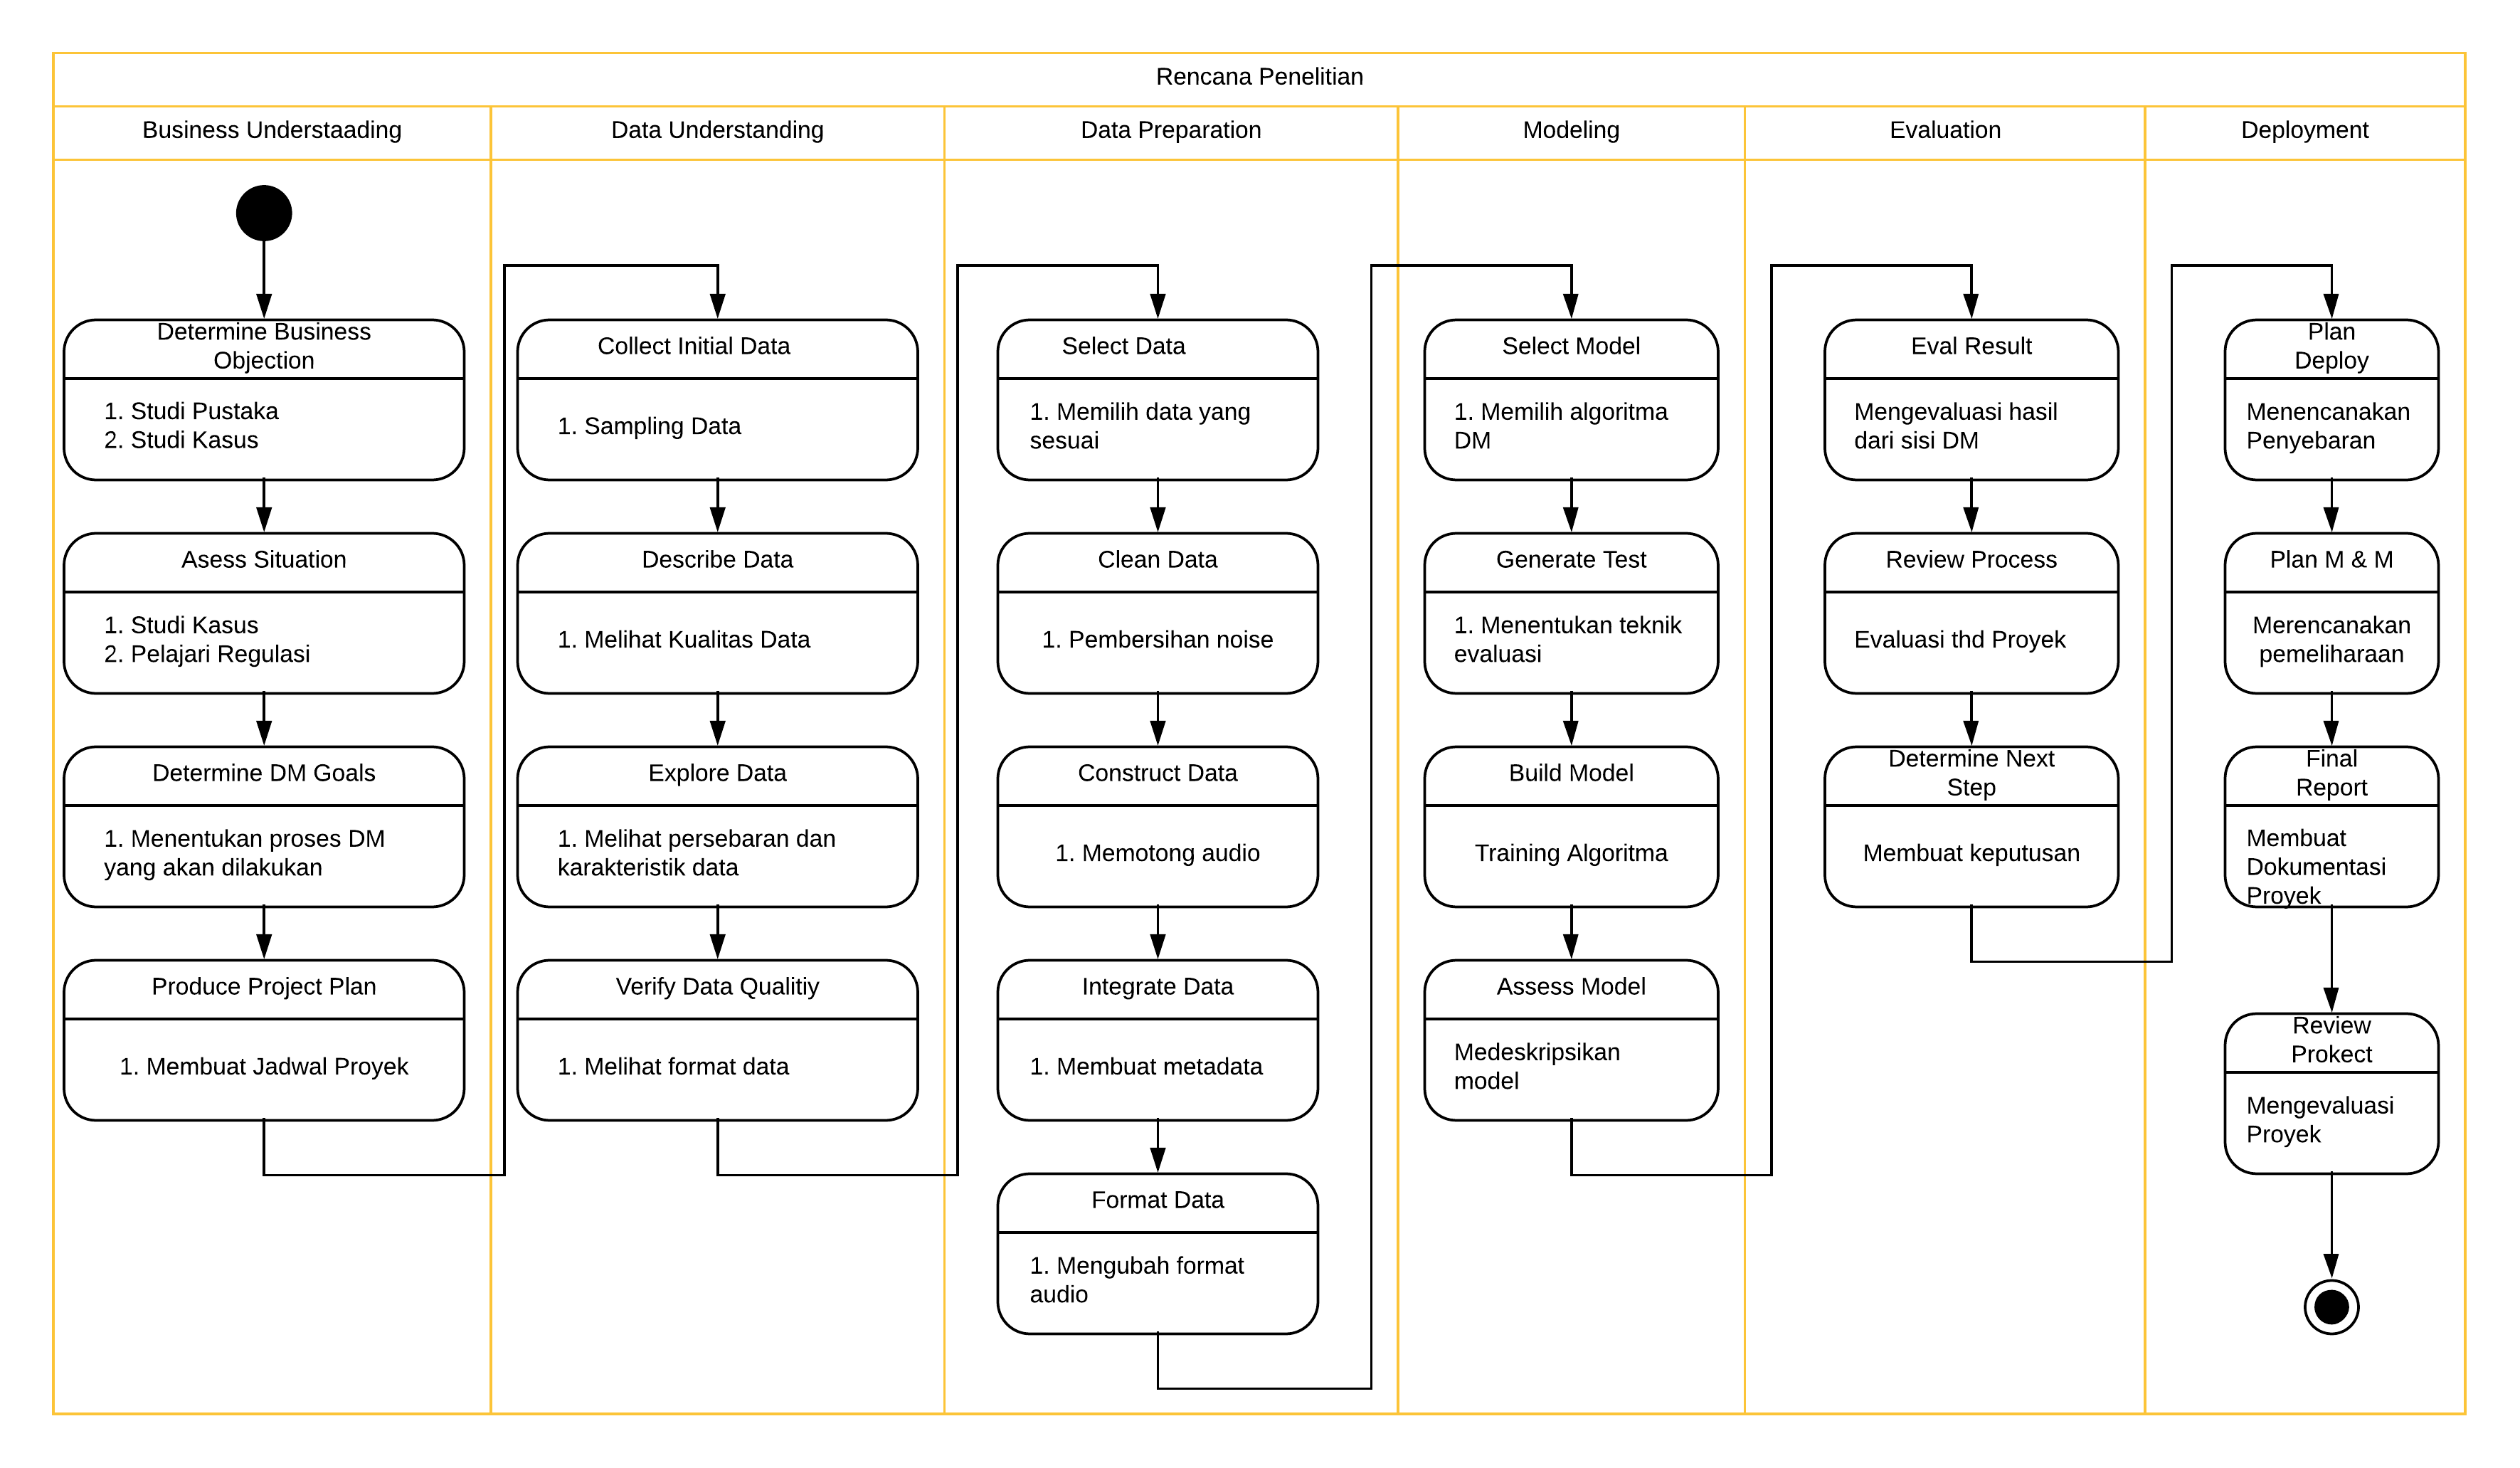
\includegraphics[width=1\linewidth]{Gambar/rencana-penelitian}
	\caption{Rencana Penelitian}
	\label{fig:rencana-penelitian}
\end{figure}


\begin{enumerate}
	\item \textit{Business Understanding}\\
	Pada fase ini, akan dilakukan studi pustaka mengenai objek penelitian yang akan diteliti. Perbandingan penerapan sistem serupa juga yang telah diterapkan di beberapa bagian dunia juga akan dikaji sebagai perbandingan. Beberapa kasus penyalahgunaan identitas juga dikaji sehingga solusi yang ditawarkan diharapkan menjadi efektif. Proses \textit{data mining}  ditawarkan sebagai solusi dengan tujuan untuk menyelesaikan permasalahan yang telah dikemukakan. Beberapa kriteria keberhasilan juga ditentukan di fase ini.
	\item \textit{Data Understanding}\\
	Di fase ini dilakukan pengumpulan data awal sebagai tolok ukur kualitas data. Pada fase ini akan dilakukan pengumpulan data suara dari 20 orang responden yang dipilih menggunakan metode sampling \textit{stratified-sampling}. Metode\textit{ stratified-sampling} adalah metode pengumpulan data dengan cara membagi populasi ke dalam sub-populasi dan mengambil sejumlah sampel dari masing-masing sub populasi tersebut. Pada penelitian ini, akan dilakukan pengambilan data dengan cara merekam suara responden dengan menggunakan perangkat telepon genggam. Masing-masing responden akan diminta untuk mengucapkan angka 0 s.d. 9 sebanyak tiga kali. Responden akan diambil dari mahasiswa dan/atau dosen di lingkungan Fakultas Ilmu Komputer dengan komposisi 10 orang laki-laki dan 10 orang perempuan.
	
	\item \textit{Data Preparation}\\
	Setelah fase sebelumnya dilakukan, maka data suara yang telah dikumpulkan akan dibersihkan dan disamakan format data dari masing-masing berkas suara. Setiap berkas suara yang ada akan dilakukan formating dengan aturan sebagai berikut:
	\begin{table}[H]\label{tbl:formatdata}
		\vspace{-2em}
		\centering
		\footnotesize
		\singlespacing
		\caption{Format Data}
		\begin{tabular}{|c|l|r|}
			\hline
			\thead{No} & \thead{Atribut} & \thead{Format} \\ \hline
			1 & Format File & WAV \\ \hline
			2 & Sample Rate & 22050 Hz \\ \hline
			3 & Bit Rate & 16 bit \\ \hline
			4 & Nama File & uuid \\ \hline
			5 & Panjang Suara & 1000 ms \\ \hline
		\end{tabular}
	\vspace{-2em}
	\end{table}
	
	Proses ini dapat dilakukan dengan menggunakan aplikasi ffmpeg. Kemudian data tersebut dibagi menjadi data uji dan data latih dengan perbangingan 20:80. Luaran dari fase ini adalah sebuah metadata yang memetakan file suara dengan pembicara yang bersesuaian. 
	
	\item \textit{Modeling}\\
	Fase ini adalah fase membuatan model dari data yang sudah dimiliki. Fase ini termasuk didalamnya proses \textit{Feature Engineering} dan \textit{Model Building}.
	Proses \textit{Feature Engineering} akan dilakukan dengan menggunakan metode MFCC dengan jumlah koefisien yang dapat divariasikan sesuai dengan kebutuhan. Selanjutnya proses pelatihan model akan dilakukan dengan melatih model dengan menggunakan data latih yang telah ditentukan sebelumnya. Model data mining yang digunakan pada proses ini adalah model \textit{Multilayer Perceptron} dengan arsitektur yang digunakan dapat diubah sesuai hasil pelatihan.
	
	\item \textit{Evaluation}\\
	Pada fase ini dilakukan pengujian dari model yang telah dibangun di proses sebelumnya. Teknik pengujian yang digunakan pada model menggunakan \textit{False Rejected Rate}, \textit{False Acceptance Rate} dan Akurasi. Pengujian tersebut dilakukan dengan cara menggunakan model untuk memprediski data uji yang sudah disiapkan. Jika hasil yang diperoleh sudah memenuhi kriteria kesuksesan, maka dapat dilakukan fase terakhir.
	
	\item \textit{Deployment}\\
	Terakhir, fase deployment akan dilakukan dengan cara membangun aplikasi simulasi dengan menggunakan bahasa pemrograman Python. Pada fase ini juga dilakukan penggabungan dengan teknik OTP yang sudah disiapkan sebelumnya. Pengujian sistem pada fase ini adalah Unit Test dengan bantuan dari module unittest dari bahasa python.
\end{enumerate}

\begin{comment}
\bibliography{daftarpustaka}
\end{comment}